\documentclass{article}
\usepackage{palatino}
\usepackage{fullpage}
\usepackage[linkcolor=true]{hyperref}
\usepackage{graphicx}
\usepackage{float}


\title{\textbf{Easy Theora Programming With Etheora.}}
\author{Ribamar Santarosa, ribamar@gmail.com}
\date{October 2007}

\begin{document}

\maketitle

\textbf{Etheora} is a C library aimed to provide a straightforward API for
programming applications that encodes or decode theora videos, using ogg
as container. Etheora users don't need to know nothing about the libtheora
or libogg (and derivatives) API. 

~\\
\textit{Etheora \textbf{doesn't} have audio/speech support yet. Although  
with etheora it's possible to get the video data from a video that 
contains audio/speech, audio/speech data will be unavailable.}

\section{Installing.}

No etheora installation. Just:
\begin{enumerate}
\item download the three files (\texttt{etheora.c}, 
\texttt{etheora.h}, \texttt{etheora-int.h}), 
\item put the \texttt{.h} files in an
include-findable directory (or tell your compiler to search the download 
directory, e.g, \texttt{-Idownload\_dir} in gcc)), 
\item and add \texttt{etheora.c} to your build project (e.g. add
\texttt{download\_dir/etheora.c} to gcc command-line). 
\end{enumerate}

\textit{\textbf{But}} libtheora (development version, if your system can tell)
is required to be present in the system. Etheora will work in the
systems where libtheora works. 

\section{Encoding.}

Encoding steps: 
\begin{enumerate}
\item Declare an etheora context structure, 
\begin{verbatim}
etheora_ctx ec;
\end{verbatim}

\item Configure the encoder with \texttt{ etheora\_enc\_setup()}, e.g, 
\begin{verbatim}
etheora_enc_setup(&ec, 640, 480, ETHEORA_ASPECT_NORMAL, 
                  12, 1, fout, finfo);
\end{verbatim}
will setup to encode a 640:480, 12/1 frames per second video, with 4:3 
aspect ratio. You may change to \texttt{ETHEORA\_ASPECT\_WIDE\_SCREEN} 
to get a 16:9 aspect ratio or \texttt{ETHEORA\_ASPECT\_PRESERVE} to 
preserve the width:height ratio. In this case, $640/480 = 4/3$, the 
latter wouldn't produce difference. 

The encoded video will be written to the file descriptor 
\texttt{FILE* fout}. Debug info will be written to \texttt{FILE*
finfo}. You may want set this as your system's null device file (e.g.
\texttt{/dev/null}) as a large amount of information  can be printed. 

\item The unnexperienced theora user may jump this step. The experienced 
libtheora user has now a last chance to change \texttt{theora\_info} and
\texttt{theora\_comment} values before encoding:
\begin{verbatim}
char *vendor = "Vendor name"; 
ec.ti.target_bitrate = 200000; 
ec.tc.vendor = vendor;
/*etc*/
\end{verbatim}
Or just maintain the default values assigned by etheora when
configuring. 

\item Start the encoder engine: 
\begin{verbatim}
etheora_enc_start(&ec); 
\end{verbatim}

\item Draw a frame. For e.g, to draw in YUV colorspace, 
\begin{verbatim}
etheora_enc_yuv_draw(&ec, i, j, y_value, u_value, v_value);
\end{verbatim}
will draw the pixel in the frame coordinate $(i,j)$. 

Although libtheora deals with frames in YUV, etheora supports 
transparent drawing in RGB with another function: 
\begin{verbatim}
etheora_enc_rgb_draw(&ec, i, j, r_value, g_value, b_value);
\end{verbatim}
Other colorspace may be available in the future. 

\textbf{\textit{For the experienced theora user: }} etheora supports 
\texttt{yuv\_buffer}s of the kinds \texttt{OC\_PF\_420}, 
\texttt{OC\_PF\_422} and \texttt{OC\_PF\_444} in despite of
your libtheora version supporting them or not. Access to these
frame buffers is transparent, using the functions above. 
\texttt{etheora\_enc\_setup()} configures the encoder to use 
\texttt{OC\_PF\_420} which is the only one known to be 
supported by any libtheora version. If you're dealing with 
different chromas, you may be interested in the function 
\texttt{etheora\_resample(yuv\_buffer *source, yuv\_buffer 
*dest)} for converting them. 

\item If the frame you've just drawn \textit{isn't} the last one you
want to encode, submit it to encoding by calling: 
\begin{verbatim}
etheora_enc_nextframe(&ec);  
\end{verbatim}
Go back to draw more frames! 

\item If the frame you've just drawn \textit{is} the last one, you 
may submit it by finishing the decoding process: 
\begin{verbatim}
etheora_enc_finish(&ec);
\end{verbatim}

\end{enumerate}

And we're done. 

\section{Decoding.}

Decoding steps: 
\begin{enumerate}
\item Declare an etheora context structure, 

\begin{verbatim}
etheora_ctx ec;
\end{verbatim}

\item Configure the decoder with \texttt{ etheora\_dec\_setup()}, e.g, 
\begin{verbatim}
etheora_dec_setup(&ec, fin, finfo);
\end{verbatim}
The video will be read from the file descriptor 
\texttt{FILE* fin}. Debug info will be written to \texttt{FILE*
finfo}. You may want set this as your system's null device file (e.g.
\texttt{/dev/null}) as a large amount of information  can be printed. 

\item Start the encoder engine: 
\begin{verbatim}
etheora_dec_start(&ec); 
\end{verbatim}

\item Video info can now be known and shown: 

\begin{verbatim}
printf("video dimensions: %u:%u\n", etheora_get_width(&ec), 
                                    etheora_get_height(&ec));
printf("frame rate : %u:%u fps\n", etheora_get_fps_numerator(&ec), 
                                   etheora_get_fps_denominator(&ec));
printf("aspect ratio: %u:%u\n", etheora_get_aspect_numerator(&ec), 
                                etheora_get_aspect_denominator(&ec));
\end{verbatim}

The experienced libtheora user can read \texttt{theora\_info} and
\texttt{theora\_comment} values:
\begin{verbatim}
printf("video target bitrate: %i\n", ec.ti.target_bitrate); 
printf("vendor name: %s\n", ec.tc.vendor); 
/*etc*/
\end{verbatim}

\item Loop to obtain all frames. When \texttt{etheora\_dec\_nextframe()}
returns \textit{not zero} it can't read more data. 
\begin{verbatim}
while(etheora_dec_nextframe(&ec)){
           ...
}
\end{verbatim}

\item After decoding a frame with \texttt{etheora\_dec\_nextframe()},
frame data is available to be read. To read using YUV colorspace: 

\begin{verbatim}
etheora_dec_yuv_read(&ec, i, j, y_value, u_value, v_value);
\end{verbatim}
will draw the pixel in the frame coordinate $(i,j)$. 

Although libtheora deals with frames in YUV, etheora supports 
transparent reading in RGB with another function: 
\begin{verbatim}
etheora_enc_rgb_read(&ec, i, j, r_value, g_value, b_value);
\end{verbatim}
Other colorspace may be available in the future. 

For the experienced user, the same note shown when 
\texttt{etheora\_enc\_yuv\_draw()} and 
\texttt{etheora\_enc\_rgb\_draw()} 
were presented, in the section \textbf{Encoding}, is valid. 

\item When the decoding loop finishes, you may free the structures
with 
\begin{verbatim}
etheora_dec_finish(&ec);
\end{verbatim}

\end{enumerate}

And we're done. 


\section{Examples/Building Examples.}

$3$ simple examples can be downloaded: \texttt{encoder-example.c},
\texttt{decoder-example.c} and \\ \texttt{decoder-example-opencv.c}

\subsection{encoder-example.c}

A very simple encoder that allows you to generate videos with
mathematical functions. 

Using gcc, you can build the encoder-example with this command: 
\begin{verbatim}
gcc encoder-example.c etheora.c  -I. -ltheora -o encoder-example  
\end{verbatim}
Assuming etheora files are in the same directory as 
\texttt{encoder-example.c}. 

Then, this command:
\begin{verbatim}
./decoder-example output-video.ogg  
\end{verbatim}
will generate a video and write it to the \texttt{output-video.ogg}. 

You can open \texttt{encoder-example.c} and play with the numeric
parameters of \texttt{etheora\_enc\_rgb\_draw()}, or use 
\texttt{etheora\_enc\_yuv\_draw()} instead. Recompile the encoder and 
get different videos. 

\subsection{decoder-example.c}

A very simple decoder that does nothing but decoding video. It allows
you to read the pixels of decoded frames. 

Using gcc, you can build the decoder-example with this command: 
\begin{verbatim}
gcc decoder-example.c etheora.c  -I. -ltheora -o decoder-example
\end{verbatim}
Assuming etheora files are in the same directory as 
\texttt{decoder-example.c}. 

Then, this command:
\begin{verbatim}
./decoder-example input-video.ogg  
\end{verbatim}
will read a video from \texttt{input-video.ogg}. 

\subsection{decoder-example-opencv.c}

A very simple decoder that decodes frames and draws them in a
opencv/highgui window. It doesn't have a good performance, it's
only to provide a visible result of the decoding process. Also it
doesn't deal with the correct video frame rate, it just waits
for $100 ~ms$ after drawing a frame.  
Requires, of course, opencv/highgui present in the system. 

Using gcc, you can build the encoder-example with this command: 
\begin{verbatim}
gcc -Wall decoder-example-opencv.c etheora.c  \
  -lhighgui -lstdc++  -I.  -ltheora -o decoder-example-opencv
\end{verbatim}
Assuming etheora files are in the same directory as 
\texttt{decoder-example-opencv.c}. 

Then, this command:
\begin{verbatim}
./decoder-example-opencv input-video.ogg  
\end{verbatim}
will read a video from \texttt{input-video.ogg} and draw in a
opencv/highgui window: 

\begin{figure}[H]
\centering
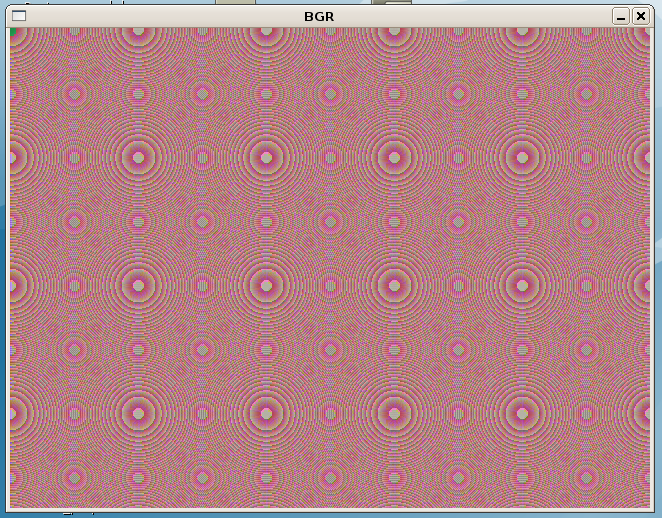
\includegraphics[scale=0.5]{opencv-hg}
\caption{\label{opencv-hg}OpenCV/Highgui window for decoding theora
videos.}
\end{figure}





\begin{verbatim}
  
\end{verbatim}

\end{document}



